%\documentclass[12pt, amstex, letterpaper] {report} %{article}


\usepackage[margin=1in]{geometry}
\topmargin -0.5in \textwidth 6.5in \textheight 9in
\footskip .5in
\headheight 0.3in


\usepackage{Sweave}

\DefineVerbatimEnvironment{Sinput}{Verbatim} {xleftmargin=0em,frame=single}
\DefineVerbatimEnvironment{Soutput}{Verbatim} {xleftmargin=0em,frame=single}

\usepackage{amssymb, mathrsfs, amsmath, amsfonts}
\usepackage{enumerate, comment}
\usepackage{hyperref, natbib,apalike, float} %cite
\usepackage{color, multirow, setspace, fancyhdr,graphicx}
\usepackage{undertilde}
\usepackage[bottom]{footmisc}
\usepackage{graphicx}
\usepackage{framed}
\usepackage{subcaption}
\usepackage{amsthm}

%\doublespacing
\pagestyle{empty}
\pagestyle{fancy}
\lhead{ }
%\rhead{May 2016}
\fancyfoot{ }
\rfoot{Dissertation $|$ \thepage}
\lfoot{Chris Vanlangenberg}
\date{}

\includecomment{comment}

\newtheorem{theorem}{Theorem}[section]
\newtheorem{defn}{Definition}[section]
\newtheorem{prop}{Proposition}
\newcommand{\pro}[1]{\begin{prop}{#1}\end{prop}}

%\newtheorem{proof}{proof}
\newtheorem{rmk}{Remark}
\newcommand{\rmark}[1]{\begin{rmk}{#1}\end{rmk}}

\numberwithin{equation}{section}
\renewcommand{\footrulewidth}{0.1pt}
\renewcommand{\headrulewidth}{0.1pt}


\newcommand{\eqn}[1]{\begin{equation}{#1}\end{equation}}

\newcommand{\beq}{\begin{equation}}
\newcommand{\eeq}{\end{equation}}
%\renewcommand\refname{Literature}
\newcommand{\blue}[1]{\textcolor{blue}{\emph{#1}}}
\newcommand{\red}[1]{\textcolor{red}{\emph{#1}}}
\newcommand{\twoc}[2]{{\textcolor{blue}{#1}} and {\textcolor{red}{#2}}}


\newcommand{\xn}{x_1,\ldots, x_n}
\newcommand{\Xn}{X_1,\ldots, X_n}
\newcommand\floor[1]{\lfloor{#1}\rfloor}
\newcommand\ceil[1]{\lceil{#1}\rceil}

\newcommand{\X}{\mathcal{X}}
\newcommand{\Sp}{\mathbb{S}}
\newcommand{\R}{\mathbb{R}}
\newcommand{\C}{\mathbb{C}}
\newcommand{\pd}{positive definite }



\newcommand{\code}[1]{{\small\texttt{#1}}}
\newcommand{\pkg}[1]{{\normalfont\textsf{#1}}}
\newcommand{\var}[1] {{\normalfont\textbf{#1}}}
\newcommand{\Cm}{$C_m(\phi_P, \phi_Q)\ $}

\newcommand{\jun}{\cite{JunStein2008}}
%%
%\begin{document}

%%------------------------------------------------------------------%%
\section{Introduction}
%%------------------------------------------------------------------%%

For a stationary time series process, the covariance and variogram function estimators have been commonly used in literature. More specifically, let $X(t)$ be a stationary process with unknown constant mean $\mu$ and covariance function $C(h), h \ge 0$. Let $\gamma(h) = C(0) - C(h)$ be the variogram function. For simplicity, we assume $\{X(t_k), k = 1, 2, \ldots, n\}$ is a sequence of random variables observed on gridded locations $\{t_k = (k-1)\delta, k \ge 1\}$ in $\R^1$ with $\delta = t_k - t_{k-1} > 0$ be the fixed interval length. First, note that $\bar{X} = \frac{1}{n}\sum_{k=1}^n X(t_k)$ is an unbiased estimator of $\mu$, and further under the certain ergodic condition, for example, the covariance function converges to zero as the lag $h \to \infty$, one has
\[
var(\bar{X}) \to 0, \quad \quad \mbox{as $n \to \infty$,}
\]
implying the consistency of $\bar{X}$ when estimating $\mu$.  \\

The covariance and variogram function estimators based on the method of moments (MOM) are given by
\begin{eqnarray*}
\hat{C}(h) &=& \frac{1}{n-h}\sum_{j = 1}^{n-h}(X(t_j+h) - \bar{X})(X(t_j) - \bar{X}), \quad \quad h = 1, 2, \cdots, n-1.  \\
2\hat{\gamma}(h) &=& \frac{1}{n-h}\sum_{j = 1}^{n-h}(X(t_j+h) - X(t_j))^2, \quad \quad h = 1, 2, \cdots, n-1,
\end{eqnarray*}
respectively. It has been shown, for example, \cite{Cressie1993}, that both the variogram and covariance MOM estimators are biased while the bias for the covariance MOM estimator is of the rate of $O(1/n)$ but the bias for the variogram MOM estimator is smaller. Furthermore, the asymptotic joint Gaussianity of the estimators $\{\hat{C}(h)\}$ and $2\hat{\gamma}(h)$ has also been established under the same ergodic conditions ({\em i.e.}, conditions that ensure the dependence in the process dies off sufficiently quickly as lag distance increases). Finally, for fixed $h$, both the variances and covariances of $\{\hat{C}(h)\}$ and of $2\hat{\gamma}(h)$ can be found (for example, in \cite{fuller2009introduction} and \cite{cressie1985fitting}) are of $O(1/n)$, which demonstrates the consistency of both estimators. Parallel results can also be obtained for the covariance and variogram MOM estimators in $\R^d$ (\cite{Cressie1993}). 

There are two distinct asymptotics in spatial statistics: increasing domain asymptotics, where more data are collected by increasing the domain, and fixed-domain or infill asymptotics, where more data are collected by sampling more densely in a fixed domain. Asymptotic properties of estimators are quite different under the two asymptotics. The above asymptotics in the time series and $\R^d$ belongs to the first one. There have been an extensive discussion of the infill asymptotics in literature, for example, \cite{Zhang:2004:IEA} showed that for the popularly used Mat\'{e}rn covariance model, one cannot correctly distinguish between two Mat\'{e}rn covariances with probability one no matter how many sample data are observed in a fixed region. Consequently, not all covariance parameters in Mat\'{e}rn models are consistently estimable. However, there seems lacking of discussions about the asymptotics on the circle and sphere. In particular, with the increasing interest in the study of the global data on the sphere, it is necessary that the infill asymptotics of the existing estimators need to be examined. As the first step for the study of the asymptotics of covariance and variogram estimators on the sphere, we consider their asymptotics on the circle. 

This chapter is organized as follow. We first introduce the random processes on the circle and then give the spectral representation of the covariance and variogram functions for stationary processes. Under the assumption of stationary Gaussian process on the circle, we show that the unbiased estimator $\bar{X}$ is not consistent when estimating $\mu$. Then, we demonstrate that the covariance function estimator based on MOM is biased with non-estimable bias, while the variogram MOM estimator is unbiased but inconsistent. Our results are supplemented via simulations.\\


%%------------------------------------------------------------------%%
\subsection{Random Process on a Circle}
%%------------------------------------------------------------------%%


Let $X(t)$ be the random process on the unit circle $\Sp^1$. If $X(t)$ is further assumed to be with finite second moment and continuity in quadratic mean, then $X(t)$ can be represented in a Fourier series which is convergent in quadratic mean (\cite{DUFOUR1976107}),
\[
X(t) = A_0 + \sum_{n=1}^\infty (A_n\cos(nt) + B_n \sin(nt)), \quad \quad t \in \Sp^1,
\]
where
\begin{eqnarray*}
A_0 = \frac{1}{2\pi}\int_S X(t)dt, \quad A_n = \frac{1}{\pi}\int_S X(t)\cos(nt)dt, \quad B_n = \frac{1}{\pi}\int_S X(t)\sin(nt)dt.
\end{eqnarray*}

Let $s, t \in S^1$. The covariance function $C(s, t)$ of the process $X(t)$ on the given locations $s$ and $t$ is given below
\begin{eqnarray*}
C(s, t) = cov(X(s), X(t)).
\end{eqnarray*}
Now we assume the underlying process $X(t)$ is stationary on the circle, that is, $E(X(t)) = \mu$ unknown, and its covariance function solely depends on the angular distance $\theta$
\[
C(\theta) = cov(X(t+\theta), X(t)), \quad \quad \theta \in [0, \pi].
\]
Under the assumption of stationarity, we have
\begin{eqnarray*}
cov(A_n, A_m) = cov(B_n, B_m) = a_n \delta(n, m), \quad\quad \mbox{and} \quad cov(A_n, B_m) = 0, \quad \mbox{for $n \ge 0, m > 0$},
\end{eqnarray*}
with $a_n \ge 0$, under which the covariance function $C(\theta)$ can be written as the following spectral representation
\begin{eqnarray*}
C(\theta) = a_0 + \sum_{n=1}^\infty a_n \cos(n\theta), \quad \quad \mbox{for $\theta \in [0, \pi]$}.
\end{eqnarray*}
By the orthogonality of $\{\cos(n\theta), n = 0, 1, 2, \cdots,\}$ on $\theta \in [0, \pi]$, we have
\[
a_0 = \frac{1}{\pi}\int_0^\pi C(\theta)d\theta, \quad \quad a_n = \frac{2}{\pi}\int_0^\pi C(\theta)\cos(n\theta)d\theta, \quad n \ge 1.
\]
If a random process $X(t)$ is intrinsically stationary, one has $E(X(t)) = \mu$, an unknown constant, as well as the variogram function depends only on the angular distance $\theta$, given by
\begin{eqnarray*}
\gamma(\theta) = var(X(t+\theta) - X(t)), \quad \quad t \in \Sp^1.
\end{eqnarray*}
Note that if $X(t)$ is stationary, then
\[
\gamma(\theta) = C(0) - C(\theta).
\]
Equivalently, $\gamma(\theta)$ has the following spectral representation
\[
\gamma(\theta) = \sum_{n = 1}^\infty a_n (1 - \cos(n\theta)).
\]



%-------------------------------------%
\subsection{Mean and Covariance Estimation on The Circle}
%-------------------------------------%

We now consider the estimation on the unknown mean $\mu$ and covariance function $C(\theta)$. Let $\{X(t_k), k = 1, 2, \cdots, n\}$ be a collection of gridded observations on the unit circle, with $t_k = (k-1)*2\pi/n, k = 1, 2, \cdots, n$. For simplicity, let $n = 2N$ be an even number. Denote $\utilde{X} = (X(t_1), X(t_2), \cdots, X(t_n))^T$ as the observed random vector. When the underlying process $X(t)$ is stationary on the unit circle, the variance-covariance matrix of $\utilde{X}$ given by

\begin{eqnarray*}
	\Sigma &=& \left(\begin{array}{ccccccc}
	C(0)      & \cdots & C((N-1)\delta ) & C(\pi) &  C((N-1)\delta ) & \cdots & C(\delta) \\
	C(\delta) & \cdots & C((N-2)\delta) & C((N-1)\delta) &  C(\pi)  & \cdots & C(2\delta) \\
	C(2\delta) & \cdots & C((N-3)\delta) & C((N-2)\delta) &  C((N-1)\delta) & \cdots & C(3\delta)\\
	\vdots    & \vdots  & \vdots  & \vdots  & \vdots  & \vdots  & \vdots  \\
	C(\delta) & \cdots & C(\pi) &  C((N-1)\delta) & C((N-2)\delta)  & \cdots & C(0)
	\end{array} \right)
\end{eqnarray*}

\noi is a symmetric circulant matrix with elements
\[
C(0),C(\delta), C(2\delta), \cdots, C((N-1)\delta), C(\pi),  C((N-1)\delta), \cdots, C(\delta), \mbox{ where } \delta = 2\pi/n.
\]
Therefore the sample mean, 
\[
\bar{X} = \frac{1}{n}{\bf 1}_n^T \utilde{X}
\]

\noi is an unbiased estimator of $\mu$ with the variance given by

\begin{eqnarray*}
var(\bar{X}) &=& cov\left(\frac{1}{n}{\bf 1}_n^T \utilde{X}, \frac{1}{n}{\bf 1}_n^T \utilde{X}\right) \nonumber \\
	&=& \frac{1}{n^2}{\bf 1}_n^T \Sigma {\bf 1}_n \nonumber \\
	&=& \frac{1}{n} \left(C(0)+C(\pi)+2 \sum_{m=1}^{N-1}C(m 2\pi/n)\right). \nonumber
\end{eqnarray*}

If we assume that $C(\theta)$ is a continuous function on $[0, \pi]$ and note the summation in the last quantity is a trapezoid sum of $C(\theta)$ on the gridded locations within $[0, \pi]$, then,
\[
\frac{1}{\pi} \frac{\pi}{2 N} \left(C(0) + \sum_{m=1}^{N-1}C(m 2\pi/n) + C(\pi) \right) \to \frac{1}{\pi} \int_0^\pi C(\theta)d\theta = a_0,
\]
as $n \to \infty$. That is, $var(\bar{X}) \to a_0$ as $n \to \infty$. Therefore, we have the following proposition. \\

\pro{ \label{prop3.1}
The sample mean $\bar{X}$ is an unbiased estimator of $\mu$ with the asymptotic variance of $a_0$. If $a_0 > 0$ and $X(t)$ is further assumed to be Gaussian, then $\bar{X}$ is NOT a consistent estimator of $\mu$.
}


\begin{proof}

It is only necessary to prove the second part. If $X(t)$ is Gaussian, then $\bar{X} \sim N(\mu, var(\bar{X})) \Rightarrow Z = \frac{\bar{X} - \mu}{\sqrt{var(\bar{X})}} \sim N(0, 1)$. First, for a fixed $\varepsilon_0 > 0$ and $\varepsilon_0 < a_0$, there exists $K$, such that for all $n > K$, we have
\[
|var(\bar{X}) - a_0| < \varepsilon_0 \Rightarrow a_0 - \varepsilon_0 < var(\bar{X}) < a_0 + \varepsilon_0.
\]
Now for each fixed $\varepsilon > 0$ and all $n > K$,
\begin{eqnarray*}
P\left(|\bar{X} - \mu| > \varepsilon\right) &=& P\left(\frac{|\bar{X} - \mu|}{\sqrt{var(\bar{X})}} > \frac{\varepsilon}{\sqrt{var(\bar{X})}} \right) \\
&\ge& P\left(|Z| > \frac{\varepsilon}{\sqrt{a_0 - \varepsilon_0}} \right) > 0.
\end{eqnarray*}
Hence $\bar{X} \not\to \mu$ in probability. The last inequality above is due to the following.
\[
\left\{|Z| > \frac{\varepsilon}{\sqrt{a_0 - \varepsilon_0}} \right\} \subseteq \left\{|Z| > \frac{\varepsilon}{\sqrt{var(\bar{X})}}\right\}.
\]

\end{proof}


\vskip 8pt

\rmark{Under the assumption of Gaussianity, Proposition \ref{prop3.1} indicates that $\bar{X}$ will never be a consistent estimator for $\mu$, which contrasts to the result given in time series and $\R^d$.}



\rmark{\label{remark2} Recall that, if $X(t)$ is stationary process on the circle, we have
\[
a_0 = var(A_0)
\]
and $\mu = E(A_0)$. Therefore, $a_0 = 0 \Rightarrow \mu = 0$, under which $var(\bar{X}) \to 0$ and so $\bar{X}$ is consistent. In other words, if $X(t)$ is a zero mean stationary process on the circle, then $\bar{X}$ is an unbiased and consistent estimator of $\mu = 0$.}

\rmark{If in practice, we have multiple copies of data observations on the circle, we can then estimate $a_0$ or $var(\bar{X})$ through these copies. More explicitly, suppose that we have {\em i.i.d.} copies of the random samples on the circle with averages denoted as $\{\bar{X}_i, i = 1, 2, \cdots, m\}$. We then use the method of moments for estimating $a_0$, which is given as following:
\[
\hat{a}_0 = \frac{1}{m-1} \sum_{j=1}^m (\bar{X}_j - \bar{\bar{X}})^2,
\]
\noi where $\bar{\bar{X}} = \frac{1}{m} \sum_{k = 1}^m \bar{X}_k$. Under some regularity conditions, one can show that $\hat{a}_0$ is a unbiased and consistent estimator of $a_0$.}

%-------------------------------------%
\section{Data Generation on a Circle}
%-------------------------------------%

To explore the properties of the MOM estimator, we perform a simple simulation study. We consider two covariance functions that are valid on a circle; exponential family and power family as given below.
\begin{eqnarray}
\label{exp_cov}
C(\theta) &=& C_1e^{-a|\theta|} \quad a>0, C_1>0, \theta \in [0, \pi], \\
\label{power_cov}
C(\theta) &=& c_0 - (|\theta|/a)^{\alpha} \quad a>0, \alpha \in (0,2].
\end{eqnarray}
\noindent where $\theta \in [0,\pi]$ and  $c_0 > 0$ satisfies $c_0 \ge \int_0^\pi(\theta/a)^{\alpha} \sin \theta d \theta$ \\

%\begin{figure}
%	\centering
%	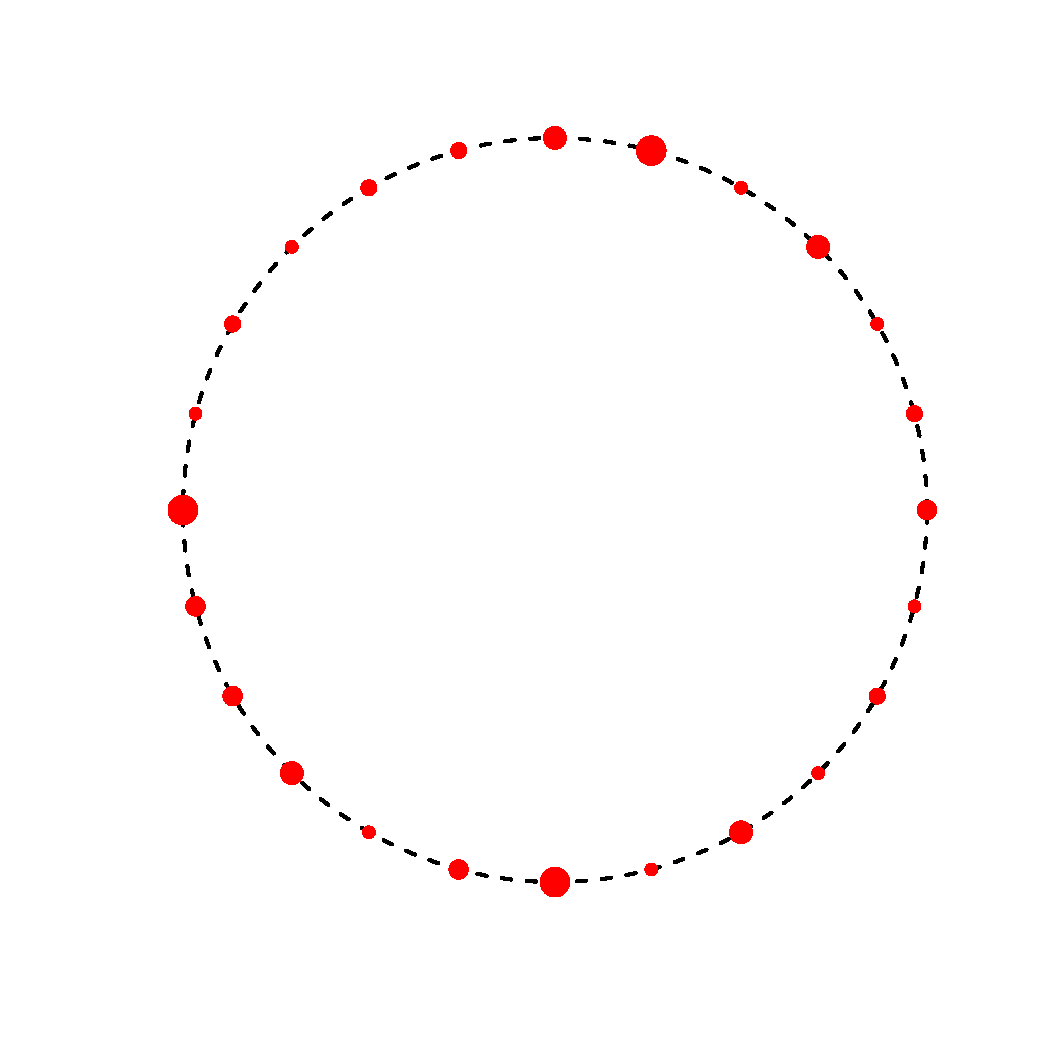
\includegraphics[width=0.5\textwidth]{graphs/process_circle}
%	\caption {Random process on a circle at 24 points ($\Delta\lambda = 15^0$), the red dots represent the  observed values at a given time and each point is associated with a random process of its own.}
%\end{figure}

Recall that $\utilde{X} = (X(t_1), X(t_2), \ldots, X(t_n))^T$ is the observed gridded data on the circle. Its variance-covariance matrix $\Sigma$ is symmetric and circulant. Hence it can be 
decomposed as
\[
\Sigma = Q \Lambda Q^T,
\]
where $\Lambda=\mbox{diag}\{\lambda_1, \lambda_2,\cdots,\lambda_n\}$ and $Q=\{\psi_1, \psi_2,\cdots,\psi_n\}$ with $\lambda_i, i = 1, 2 \ldots, n$, are eigenvalues and $\psi_1, \psi_2,\cdots,\psi_n$ are eigenvectors of the circulant matrix, respectively. (See Section 1.3). Therefore, let $\utilde{Z}$ be {\em i.i.d.} standard normal random variates, then
\[
	\utilde{X} = \Sigma^{1/2}*\utilde{Z} = Q\Lambda^{1/2}Q^T*\utilde{Z},
\]
\noi is the observed data vector that follows the given covariance function.

%-------------------------------------%
\section{Covariance MOM Estimator}
%-------------------------------------%

% \beq\label{cov:circle1}
% C(\theta) = \frac{1}{n_L} \sum_{i=1}^{n_L} (X(a_i+\theta)\cdot X(a_i))-(\overline{X(a)})^2
% \eeq
%\vskip 8pt

Now we consider the MOM estimator of $C(\theta)$, which is given by
\beq \label{covarince_estimator}
\hat{C}(\Delta \lambda) = \frac{1}{n}\sum_{i = 1}^n (X(t_i + \Delta \lambda) - \bar{X})(X(t_i) - \bar{X}),
\eeq

\noi where $\Delta \lambda = 0, 2\pi/n, 4\pi/n, \cdots, 2(N-1)\pi/n$ (for simplicity, we set n=2N even). \\

For simulation, we set $C_1 = a = 1$ and choose $\alpha = 0.5$, $c_0 \ge \int_0^\pi(\theta)^{0.5} \sin(\theta) d\theta$. From Fresnel integral, it can be shown that $c_0 \ge 2.4353$. Now we compare the covariance estimator (empirical) to its theoretical covariance given by \eqref{exp_cov} and \eqref{power_cov}, respectively. We computed the MOM estimator $\hat{C}(\theta)$ with $n = 48$ gridded observations on the circle with 500 repetitions.

      \begin{figure}[H]
      	\centering
       	% 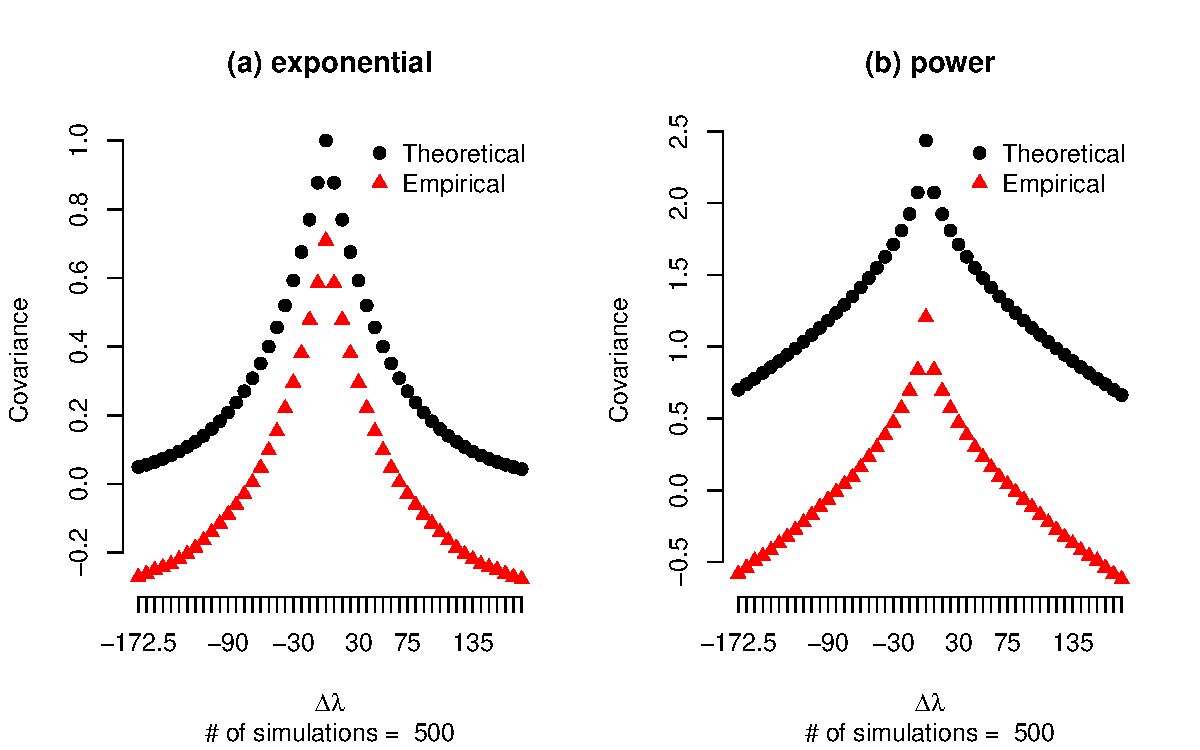
\includegraphics[width=0.9\textwidth]{graphs/covarince_circle}
       	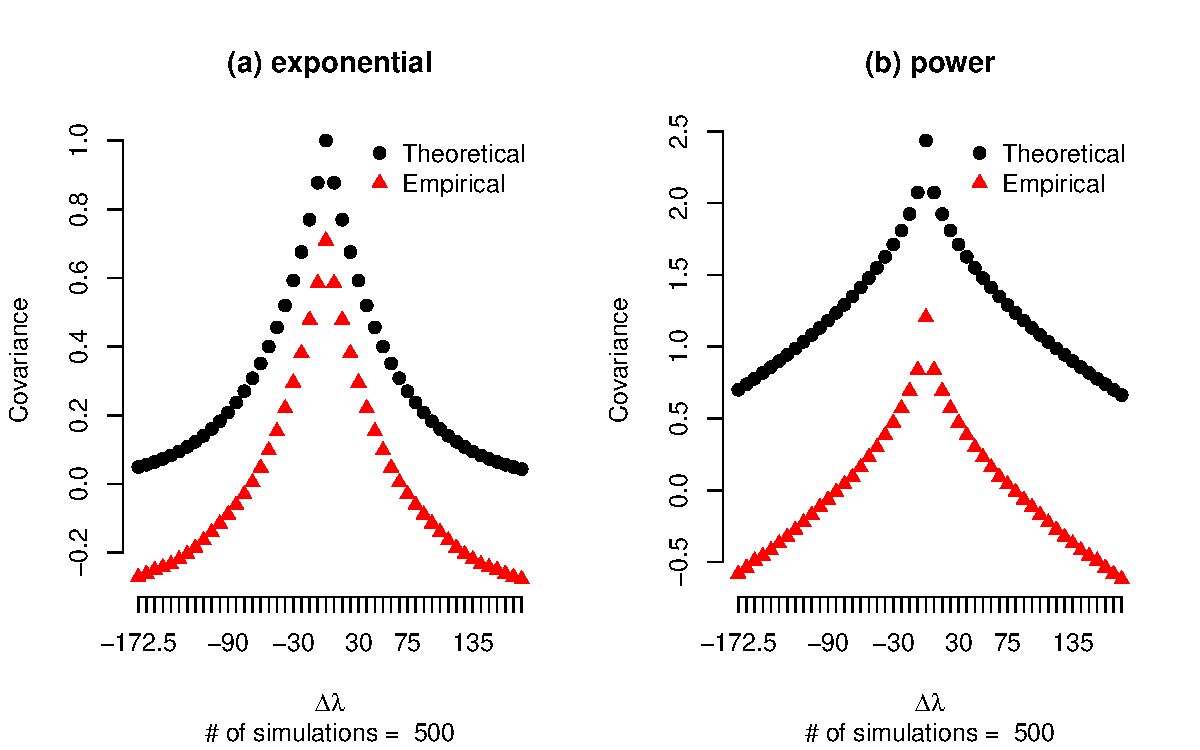
\includegraphics[keepaspectratio, scale = .8]{graphs/covariance_circle.pdf}
      	\caption[Comparison Between Theoretical and Empirical Covariance Without] {Comparison between theoretical and empirical covariance without any adjustments, on a circle. }
      	\label{covariance_circle}
      \end{figure}
% and it is easy to notice a shift appearing in both graphs.
\rmark{ One can easily notice a shift between theoretical can empirical values appearing on both graphs (Figure \ref{covariance_circle}). The shift  can be shown to be approximately equal to $a_0$, where $a_0 = \frac{1}{\pi}\int_0^\pi C(\theta)d\theta$. For both covariance functions considered, we can obtain	
\begin{eqnarray*}
	    \mbox{exponential : }  	a_0 &=& \frac{C_1}{a\pi}(1 - e^{-a\pi}), \\
	    \mbox{power : }  	a_0       &=& c_0 - \left(\frac{\pi}{a}\right)^{\alpha}\frac{1}{\alpha + 1}.
\end{eqnarray*}
}
Now we consider the following covariance function, after subtracting $a_0$ from $C(\theta)$.
	      \[
	      	D(\theta) = C(\theta) - a_0.
	      \]
From Remark \ref{remark2}, $D(\theta)$ is now the covariance function of a zero mean stationary process on the circle. The simulation setup is the same as above except that $C(\theta)$ is replaced with $D(\theta)$. The results show that both empirical and theoretical values match very well (Figure \ref{covariance_remove_a0}). 

	      \begin{figure}
	      	\centering
	      	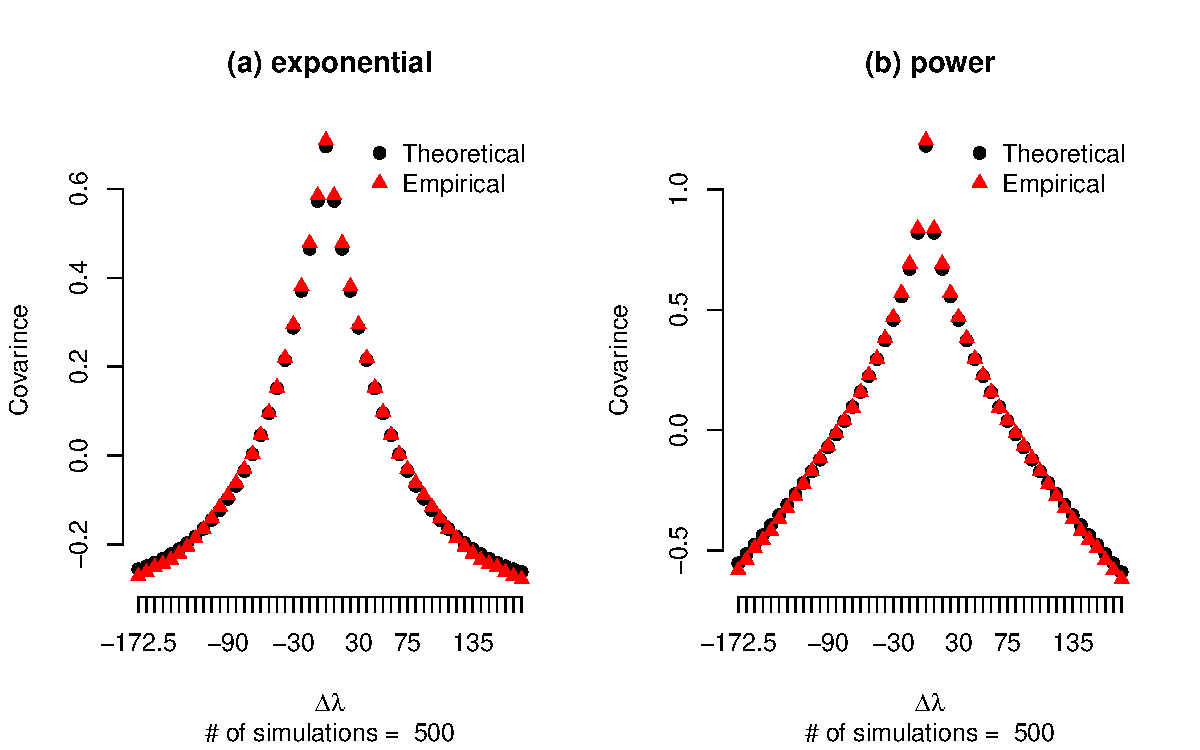
\includegraphics[width=0.8\textwidth]{graphs/covarince_circle_remove_a0}
	      	% 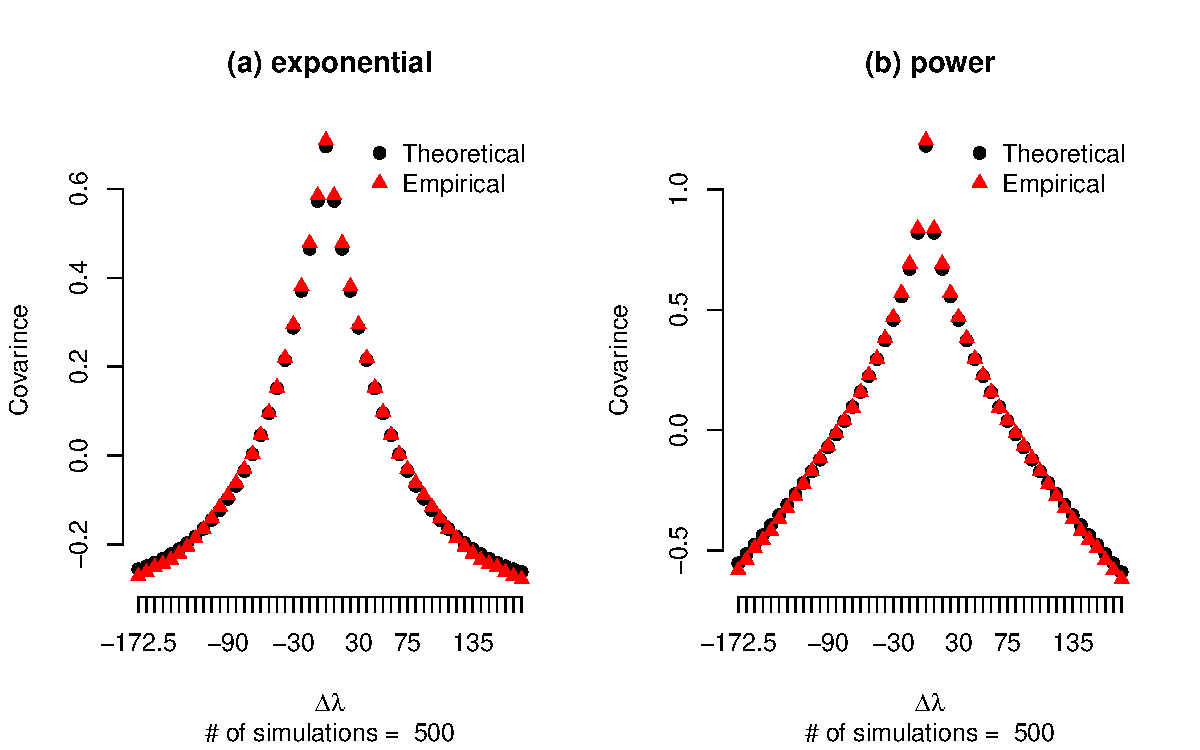
\includegraphics[scale=.8, keepaspectratio]{graphs/covarince_circle_remove_a0.pdf}
	      	%graph from data genaration summary doc line 194
	      	\caption[Theoretical and Empirical Covariance Comparison on a Circle Using The]{Theoretical and empirical covariance comparison on a circle using the modified covariance function $D(\theta)$.}
	      	\label{covariance_remove_a0}
	      \end{figure}

\rmark{ The covariance estimator is biased and the bias is close to $a_0$, which is non-estimable. However if {\em i.i.d.} copies of random data on the same circle are available then one can estimate $a_0$ {\em i.e.}, $\hat{a} = var(\bar{X})$. The new covariance estimator could then be estimated by subtracting $\hat{a_0}$ form the original MOM estimator as given below.
\[
\hat{C}(\Delta \lambda) = \left( \frac{1}{n}\sum_{i = 1}^n (X(t_i + \Delta \lambda) - \bar{X})(X(t_i) - \bar{X}) \right) -  \hat{a_0}.
\]
}

Our simulation shows both curves match very well (Figure \ref{covariance_estimate_a0}).
	
	\begin{figure}[H]
	 \centering
	 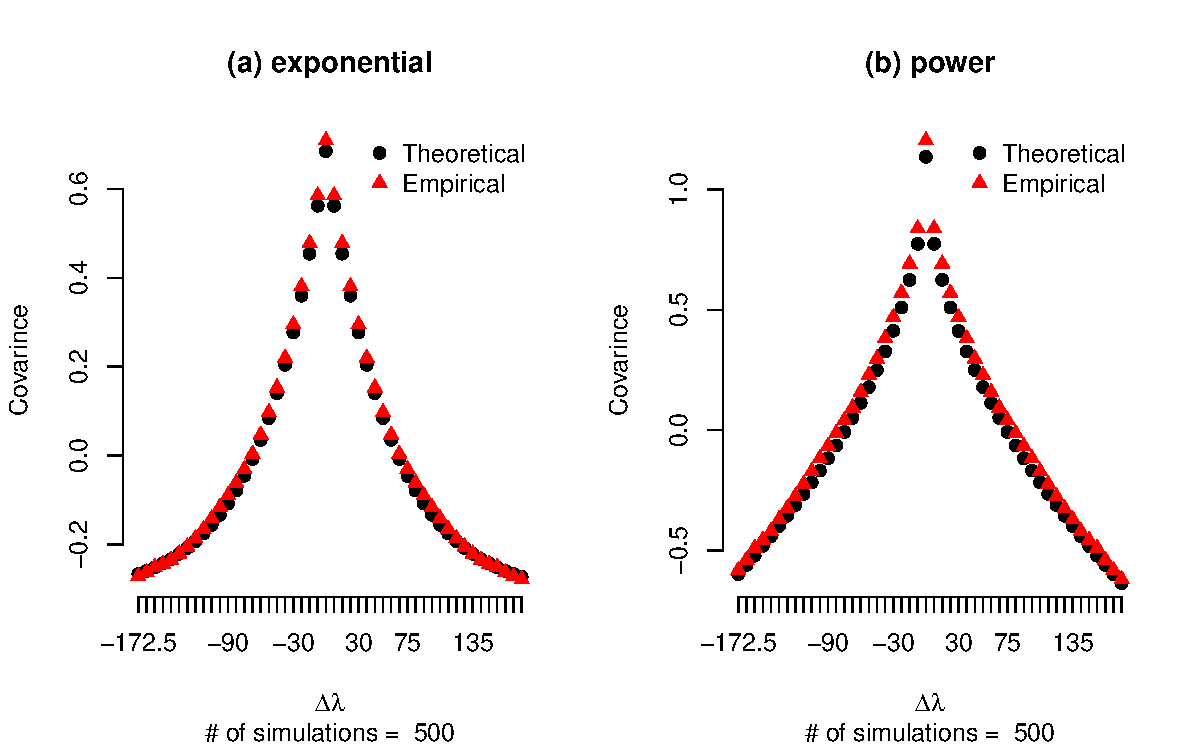
\includegraphics[width=0.8\textwidth]{graphs/covarince_circle_estimate_a0}
	 % \includegraphics[scale=.8, keepaspectratio]]{graphs/covarince_circle_estimate_a0}
	 %graph from data genaration summary doc line 194
	 \caption[Theoretical and Empirical Covariance Comparison on a Circle After]{Theoretical and empirical covariance comparison on a circle after substrating $\hat{a_0}$ from empirical covariance.}
	 \label{covariance_estimate_a0}
	 \end{figure}


Now we theoretically calculate the unbiasedness and consistency of the above estimator.

\begin{eqnarray*}
	E(\hat{C}(\Delta \lambda)) &=& \frac{1}{n}\sum_{i = 1}^n E((X(t_i + \Delta \lambda) - \bar{X})(X(t_i) - \bar{X})) \\
	&=& \frac{1}{n}\sum_{i = 1}^n E((X(t_i + \Delta \lambda) - \mu - (\bar{X} - \mu))(X(t_i) -\mu - (\bar{X}) - \mu)) \\
	&=& \frac{1}{n}\sum_{i=1}^n cov(X(t_i+\Delta \lambda), X(t_i)) - \frac{1}{n}\sum_{i = 1}^n E((X(t_i + \Delta \lambda) - \mu)(\bar{X} - \mu)) \\
	& & -\frac{1}{n}\sum_{i = 1}^n E((X(t_i) - \mu)(\bar{X} - \mu)) + \frac{1}{n}\sum_{i = 1}^n E((\bar{X} - \mu)(\bar{X} - \mu)) \\
	&=& C(\Delta \lambda) -E((\bar{X} - \mu)(\bar{X} - \mu)) - E((\bar{X} - \mu)(\bar{X} - \mu)) \\
	& & + E((\bar{X} - \mu)(\bar{X} - \mu)) \\
	&=& C(\Delta \lambda) - var(\bar{X}).
\end{eqnarray*}

That is, the MOM estimator $\hat{C}(\Delta \lambda)$ of the covariance function is actually a biased estimator with the shift amount approximately equal to $a_0$ unless $a_0 = 0$. In other words, if $a_0 = 0$, the MOM estimator $\hat{C}(\Delta \lambda)$ is an unbiased estimator of $C(\theta)$. In summary, we have \\

\pro{\label{prop3.2}
The MOM covariance estimator is a biased estimator of the true covariance function $C(\theta)$, if $a_0 > 0$. However, if the process is a zero mean process then the MOM covariance estimator is unbiased.
}

%-------------------------------------%
\section{Variogram MOM Estimator}
%-------------------------------------%

When the random process on a circle is stationary, the semivariogram can be obtained by
\[
\gamma(\theta) = C(0) - C(\theta),
\]

In $\R^n$, The variogram MOM estimator generally performs better than the covariance MOM estimator \cite{Cressie1993}. Given gridded data observations $\utilde{X}$, the variogram MOM estimator is given by
\beq
\hat{\gamma}(\Delta \lambda) = \frac{1}{2n} \sum_{i=1}^n (X(t_i + \Delta \lambda) - X(t_i))^2.
\eeq

We first perform the simulation with the same set up as before. Note that the theoretical exponential and power variogram functions are given below.
\begin{eqnarray*}
	\mbox{exponential : }\gamma(\theta) &=& C(0) - C(\theta) = C_1(1-e^{-a|\theta|}), \\
	\mbox{power : } \gamma(\theta) &=& C(0) - C(\theta) = (|\theta|/a)^{\alpha}.
\end{eqnarray*}

We computed the variogram estimator $\hat{\gamma}(\theta)$ with $n = 48$ gridded observations on the circle with 500 repetitions and then compare them with the theoretical values. One can see that both empirical and theoretical values match very well (Figure \ref{variogram_circle}).


\begin{figure}[H]
	\centering
	%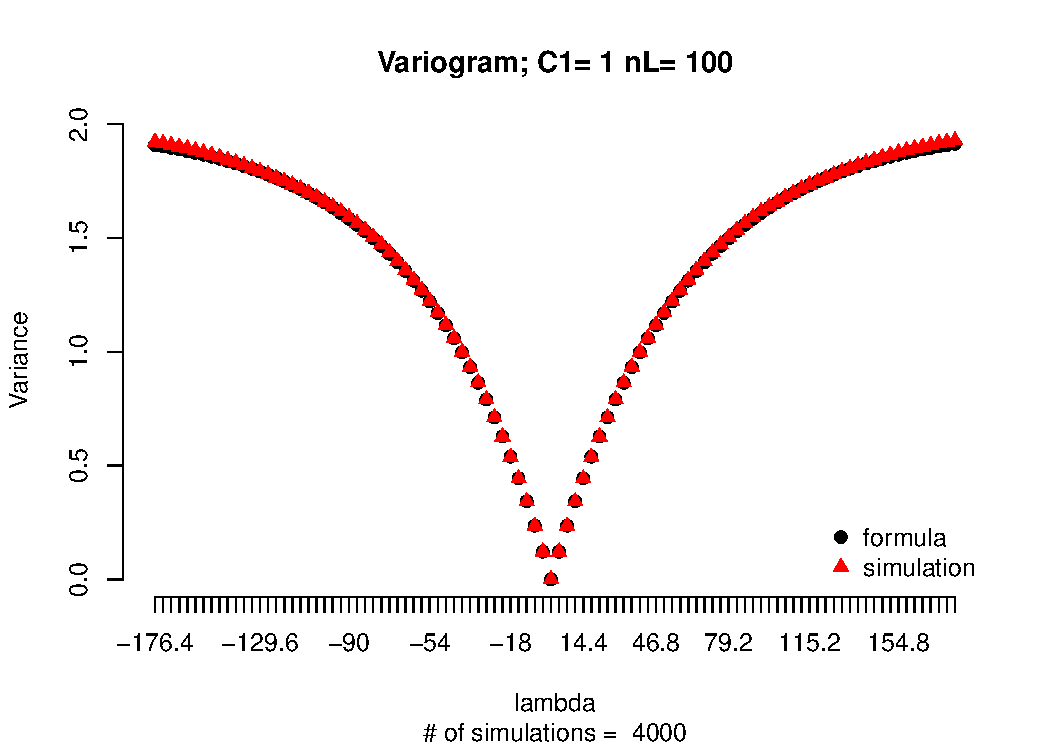
\includegraphics[width=0.65\textwidth]{graphs/variogram_plot_4000}
	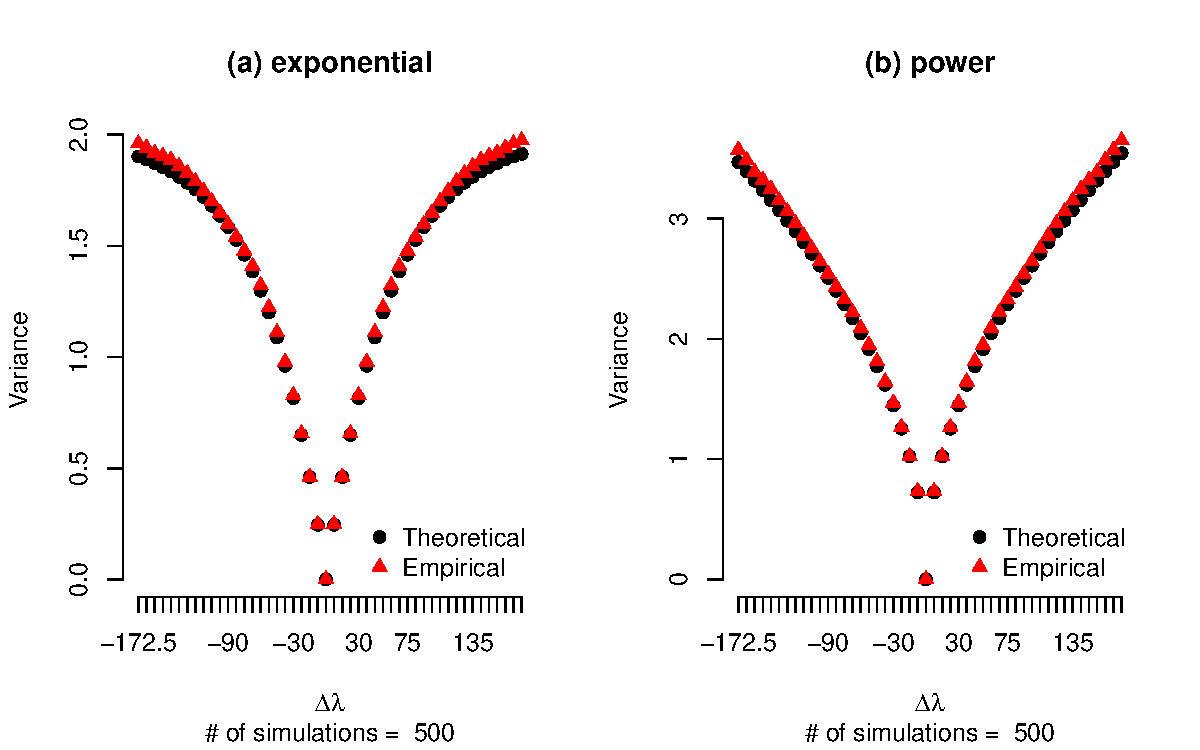
\includegraphics[width=0.9\textwidth]{graphs/variogram_plot_500}
	%graph from data genaration summary doc line 177
	\caption[Comparison Between Theoretical and Empirical Variogram on a Circle.]{Comparison between theoretical and empirical variogram on a circle.}
	\label{variogram_circle}
\end{figure}


%-------------------------------------%
%\subsection{Variogram estimation}
%-------------------------------------%


Now we explore the asymptotics of the MOM variogram estimator.

\begin{eqnarray*}
E(\hat{\gamma}(\Delta \lambda)) &=& \frac{1}{2n} \sum_{i = 1}^n E(X(t_i + \Delta \lambda) - X(t_i))^2 \\
&=& \frac{1}{2n} \sum_{i = 1}^n E((X(t_i + \Delta \lambda)-\mu) - (X(t_i) - \mu))^2 \\
&=& \frac{1}{2n} \sum_{i = 1}^n cov(X(t_i + \Delta \lambda) - X(t_i), X(t_i + \Delta \lambda) - X(t_i)) \\
&=& \frac{1}{2n} \sum_{i = 1}^n \left(cov(X(t_i + \Delta \lambda), X(t_i + \Delta \lambda)) + cov(X(t_i), X(t_i))\right. \\
& & - \left. 2cov(X(t_i + \Delta \lambda), X(t_i)) \right)\\
&=& \frac{1}{2n} \sum_{i = 1}^n \left( C(0) + C(0) - 2C(\Delta \lambda)\right) \\
&=& C(0) - C(\Delta \lambda) = \gamma(\Delta \lambda).
\end{eqnarray*}

\noi Therefore, $\hat{\gamma}(\Delta \lambda)$ is an unbiased estimator of $\gamma(\Delta \lambda)$. \\

We first calculate the variance and covariance of the variogram estimator on the circle. Again we consider the equal-distance gridded points on the circle $\{t_i: 1 \le i \le n, t_i = (i-1) \times 2\pi/n\}$ and $\utilde{X} = (X(t_1), X(t_2), \ldots, X(t_n))^T,$ being the observed data values. Assume that the random process $X(t)$ is stationary. Note that the Matheron's classical semi-variogram estimator on the circle based on the method of moments can be written as
\[
\hat{\gamma}(\Delta \lambda) = \utilde{X}^T A(\Delta \lambda)\utilde{X}.
\]
Here for all $\Delta \lambda$, $A(\Delta \lambda)$ is a circulant matrix, and in particular, $A(0)= 0$. For simplicity, we set $n = 2N$ to be even. First we give an example $n = 6$ to demonstrate the structure of $A(\Delta \lambda)$.

Let $n = 6$. We have four distance angles $\Delta \lambda = 0, \pi/3, 2\pi/3, \pi$. Then each of design matrices $A(\Delta \lambda)$ is given below.

\begin{eqnarray*}
A(0) &=& 0 ;  \\
A(\pi/3) &=& \frac{1}{12} \left(\begin{array}{cccccc}
2  &  -1 & 0  & 0 & 0 & -1 \\
-1 &  2  & -1 & 0 & 0 & 0   \\
0  & -1  & 2  & -1 & 0  & 0 \\
0  & 0   & -1 & 2  & -1 & 0 \\
0  & 0   &  0 & -1 & 2  & -1 \\
-1 & 0   &  0 &  0 & -1 & 2
\end{array}
\right) = \frac{1}{12} circ(2, -1, 0, 0, 0, -1);
\end{eqnarray*}
similarly,
\begin{eqnarray*}
A(2\pi/3) &=&  \frac{1}{12} circ(2, 0, -1, 0, -1, 0);\\
A(\pi) &=& \frac{1}{12} circ(2, 0, 0, -2, 0, 0).
\end{eqnarray*}

% \begin{eqnarray*}
% A(2\pi/3) &=& \frac{1}{12} \left(\begin{array}{cccccc}
% 2  &  0  & -1  & 0 & -1 & 0 \\
% 0  &  2  & 0   & -1 & 0 & -1   \\
% -1  & 0  & 2   & 0 & -1  & 0 \\
% 0  & -1   & 0  & 2  & 0 & -1 \\
% -1  & 0   &  -1  & 0 & 2  & 0 \\
% 0 & -1   &  0  &  -1 & 0 & 2
% \end{array}
% \right) = \frac{1}{12} circ(2, 0, -1, 0, -1, 0); \\
% A(\pi) &=& \frac{1}{12} \left(\begin{array}{cccccc}
% 2  &  0 & 0  & -2 & 0 & 0 \\
% 0 &  2  & 0 & 0 & -2 & 0   \\
% 0  & 0  & 2  & 0 & 0  & -2 \\
% -2  & 0   & 0 & 2  & 0 & 0 \\
% 0  & -2   &  0 & 0 & 2  & 0 \\
% 0 & 0   &  -2 &  0 & 0 & 2
% \end{array}
% \right) = \frac{1}{12} circ(2, 0, 0, -2, 0, 0).
% \end{eqnarray*}

In general, for $1 \le m \le N-1$, and let $\delta = 2\pi/n$ be the common interval length so that $\Delta \lambda = m\delta$. Then we have
\begin{eqnarray*}
A(0) &=& 0; \\
A(m\delta) &=& \frac{1}{2n}circ(2, 0, 0, \ldots, -1, 0, \ldots, -1, 0, \ldots, 0), \\
& & \mbox{where $-1$'s are placed at $(m+1)^{th}$ and $(n-m+1)^{th}$ positions, respectively;} \\
A(N\delta) &=& A(\pi) = \frac{1}{2n}circ(2, 0, 0, \ldots, -2, 0, \ldots, 0),\\
& & \mbox{where $-2$ is placed at $(N+1)$th position.}
\end{eqnarray*}
Obviously, $A(\Delta \lambda) = A(m\delta)$ is a symmetric circulant matrix. From Section 1.3, the eigenvalues of $A(m \delta)$ is then given by
\begin{eqnarray*}
\lambda_j^{(A)} &=& \frac{1}{2n}(2 - (\exp(j2\pi i/n))^m - (\exp(j2\pi i/n))^{n-m}) \\
&=& \frac{1}{2n}(2 - \exp(mj2\pi i/n) - \exp(-mj2\pi i/n)) \\
&=& \frac{1}{n}(1 - \cos(jm\lambda)) = \frac{1}{n}(1 - \cos(j\Delta \lambda)), \quad \quad j = 0, 1, 2, \ldots, n-1.
\end{eqnarray*}
for $1 \le m \le N-1$, and for $m = N$,

\begin{eqnarray*}
\lambda_j^{(A)} &=& \frac{1}{2n}(2 - 2 (\exp(j2\pi i/n))^{N}) \\
 &=& \frac{1}{n}(1 - \cos(j\pi)) \\
 &=& \frac{1}{n}(1 - \cos(j\Delta \lambda)), \quad \quad j = 0, 1, \cdots, n-1.
\end{eqnarray*}

In addition, from Section \ref{circulant}, all circulant matrices can be orthogonally diagonalized using the same orthogonal (Fourier) matrix, denoted as $P$. Consequently,
the trace of the product of circulant matrices is the trace of product of diagonal matrices, which is the sum of the product of corresponding eigenvalues from those circulant matrices. \\

Now we consider the distribution of the variogram estimator. First we write the variogram estimator in the following form
\begin{eqnarray*}
\hat{\gamma}(\Delta \lambda) &=& \frac{1}{2n} \sum_{i=1}^n (X(t_i + \Delta \lambda) - X(t_i))^2  \\
&=& \frac{1}{2n} \sum_{i=1}^n ((X(t_i + \Delta \lambda)-\mu) - (X(t_i)-\mu))^2.
\end{eqnarray*}
\noi Therefore,
\beq
\hat{\gamma}(\Delta \lambda) = (\utilde{X}-\utilde{\bf 1}_n\mu)^T A(\Delta \lambda)(\utilde{X}-\utilde{\bf 1}_n\mu)
\eeq

Note that $A(\Delta \lambda)$ is a circulant matrix with following spectral decomposition
\begin{eqnarray*}
A(\Delta \lambda) &=& P \Lambda^{(A)}P^T,
\end{eqnarray*}
where $P$ is the Fourier matrix (orthonormal), solely depending on the dimension of $A$, and
\begin{eqnarray*}
\Lambda^{(A)} &=& \mbox{diag}(\lambda_1^{(A)}, \lambda_2^{(A)}, \cdots, \lambda_n^{(A)}), \\
\mbox{with} \quad \lambda_m^{(A)} &=& \frac{1}{n}(1 - \cos((m-1)\Delta \lambda)), \quad \quad m = 1, 2, \cdots, n.
\end{eqnarray*}

If $\utilde{X}$ follows a multivariate normal $N(\utilde{\bf 1}_n\mu, \Sigma)$, then $(\utilde{X}-\utilde{\bf 1}_n\mu) \sim N(\utilde{\bf 0}, \Sigma)$. Note that
the variance-covariance matrix $\Sigma$ is also a circulant matrix, which has the following spectral decomposition.
\begin{eqnarray*}
\Sigma &=& P \Lambda^{(\Sigma)} P^T,\\
\mbox{with}\quad \Lambda^{(\Sigma)} &=& \mbox{diag}(\lambda_1^{(\Sigma)}, \lambda_2^{(\Sigma)}, \cdots, \lambda_n^{(\Sigma)}),
\end{eqnarray*}
\begin{flalign*}
\text{where } \quad \lambda_j^{(\Sigma)} &= \left(C(0) + 2\sum_{m = 1}^{N-1}C(m\delta)\cos((j-1)m\delta) + C(\pi)\cos((j-1)N\delta)\right).
\end{flalign*}

Let $\utilde{Y} = P^T\left(\utilde{X} - \utilde{\bf 1}_n \mu \right)$, then $\utilde{Y}$ follows a multivariate normal distribution with mean $\utilde{\bf 0}$ and variance-covariance matrix given by
\begin{eqnarray*}
var(\utilde{Y}) &=& cov(P^T\left(\utilde{X} - \utilde{\bf 1}_n \mu \right), P^T\left(\utilde{X} - \utilde{\bf 1}_n \mu \right)) \\
&=& P^T \Sigma P  = P^T P \Lambda^{(\Sigma)} P^T P = \Lambda^{(\Sigma)}.
\end{eqnarray*}

That is, $\utilde{Y} = (Y_1, Y_2, \cdots, Y_n)^T$ are independent normal random variates with mean 0 and variance $\lambda_j^{(\Sigma)}$, $j=1,2,\ldots,n$ respectively. \\

The variogram estimator is then given by
\begin{eqnarray*}
\hat{\gamma}(\Delta \lambda) &=& (\utilde{X}-\utilde{\bf 1}_n\mu)^T A(\Delta \lambda)(\utilde{X}-\utilde{\bf 1}_n\mu) \\
&=& (P(\utilde{X}-\utilde{\bf 1}_n\mu))^T \Lambda^{(A)} (P^T(\utilde{X}-\utilde{\bf 1}_n\mu))  \\
&=& \utilde{Y} \Lambda^{(A)} \utilde{Y} = \sum_{m = 1}^n \lambda_m^{(A)} Y_m^2.
\end{eqnarray*}

Note $\frac{Y_m}{\sqrt{\lambda_m^{(\Sigma)}}} \sim N(0, 1)$, and so $\frac{Y_m^2}{\lambda_m^{(\Sigma)}} \sim \chi_1^2$ (or written as $\chi_{1, m}^2$ due to the dependency on $m$), which implies
\begin{eqnarray*}
\hat{\gamma}(\Delta \lambda) &=& \sum_{m = 1}^n \lambda_m^{(A)} \lambda_m^{(\Sigma)} \left(\frac{Y_m}{\sqrt{\lambda_m^{(\Sigma)}}}\right)^2 \stackrel{\triangle}{=} \sum_{m = 1}^n \lambda_m^{(A)} \lambda_m^{(\Sigma)} \chi_{1,m}^2.
\end{eqnarray*}
Here $\chi_{1, 1}^2, \chi_{1, 2}^2, \cdots, \chi_{1, n}^2$ are {\em i.i.d.} following $\chi_1^2$ distribution. Hence
\[
E(\hat{\gamma}(\Delta \lambda)) = \sum_{m = 1}^n \lambda_m^{(A)} \lambda_m^{(\Sigma)}, \quad \quad var(\hat{\gamma}(\Delta \lambda)) = 2 \sum_{m = 1}^n (\lambda_m^{(A)} \lambda_m^{(\Sigma)})^2
\]
After tedious calculations, one can show that
\[
E(\hat{\gamma}(\Delta \lambda)) = \sum_{m = 1}^n \lambda_m^{(A)} \lambda_m^{(\Sigma)} = \gamma(\Delta \lambda).
\]
which recovers the result we had early. Next we consider the variance of the variogram estimator under the Gaussian assumption. \\

Without loss of generality, we assume that $a_1 > 0$ (otherwise, we can always choose some $a_m$ such that $a_m > 0$). First notice that
\begin{eqnarray*}
\hat{\gamma}(\Delta \lambda) &=& \sum_{m = 1}^n \lambda_m^{(A)} \lambda_m^{(\Sigma)} \chi_{1,m}^2  \\
&=& (C(0) - C(\Delta \lambda)) \sum_{m = 1}^n \frac{\lambda_m^{(A)} \lambda_m^{(\Sigma)}}{C(0) - C(\Delta \lambda)} \chi_{1,m}^2  \\
&\overset{\bigtriangleup}{=}&  (C(0) - C(\Delta \lambda)) \sum_{m = 1}^n C_{n,m} \chi_{1,m}^2,
\end{eqnarray*}
where $\sum_{m=1}^n C_{n, m} = \sum_{m=1}^n \frac{\lambda_m^{(A)} \lambda_m^{(\Sigma)}}{C(0) - C(\Delta \lambda)} = 1$ and $C_{n, m} > 0$ since both the matrices $A$ and $\Sigma$ are positive definite. Hence
\begin{eqnarray*}
var(\hat{\gamma}(\Delta \lambda)) &=& (C(0) - C(\Delta \lambda))^2 * 2 * \left(\sum_{m = 1}^n C_{n,m}^2\right) \\
&\le& 2(C(0) - C(\Delta \lambda))^2\left(\sum_{m = 1}^n C_{n,m}\right) = 2(C(0) - C(\Delta \lambda))^2.
\end{eqnarray*}
On the other hand,
\begin{eqnarray*}
var(\hat{\gamma}(\Delta \lambda)) &=& (C(0) - C(\Delta \lambda))^2 * 2 * \left(\sum_{m = 1}^n C_{n,m}^2\right) \\
&\ge& (C(0) - C(\Delta \lambda))^2 * 2 * C_{n, 2}^2.
\end{eqnarray*}
Note that
\begin{eqnarray*}
C_{n, 2} &=& \frac{1 - \cos(\Delta \lambda)}{C(0) - C(\Delta \lambda)} \frac{1}{n}\left(C(0) + 2\sum_{k = 1}^{N-1}C(k\delta)\cos(k\delta) + C(\pi)\cos(N\delta)\right) \\
&=& \frac{1 - \cos(\Delta \lambda)}{C(0) - C(\Delta \lambda)} \frac{1}{\pi} \frac{\pi}{n}\left(C(0) + 2\sum_{k = 1}^{N-1}C(k\delta)\cos(k\delta) + C(\pi)\cos(N\delta)\right).
\end{eqnarray*}
Now we consider the limit of $C_{n, 2}$ when $n \to \infty$. We want to point out that when $n \to \infty$, we are sampling denser and denser data points over the circle so that we are always maintaining $\Delta \lambda$ to be fixed. A simple approach is to take the sample size $n$ to be doubled so that $n$ tends to infinity while maintaining $\gamma(\Delta \lambda)$ to be estimable. Under this setting, we have
\begin{eqnarray*}
\frac{\pi}{n}\left(C(0) + 2\sum_{k = 1}^{N-1}C(k\delta)\cos(k\delta) + C(\pi)\cos(N\delta)\right) \to \int_0^\pi C(\theta)\cos(\theta)d\theta, \quad \mbox{as $n \to \infty$},
\end{eqnarray*}
and so
\begin{eqnarray*}
C_{n, 2} &\to& \frac{1 - \cos(\Delta \lambda)}{C(0) - C(\Delta \lambda)} \frac{1}{2} \frac{2}{\pi}\int_0^\pi C(\theta)\cos(\theta)d\theta = \frac{1 - \cos(\Delta \lambda)}{C(0) - C(\Delta \lambda)}*\frac{a_1}{2} \\
C_{n, 2} &>& \frac{1 - \cos(\Delta \lambda)}{C(0) - C(\Delta \lambda)}*(\frac{a_1}{2} - \varepsilon_0)
\end{eqnarray*}
for a fixed $0 < \varepsilon_0 < \frac{a_1}{2}$ and a large enough sample size $n$. Consequently,
\begin{eqnarray*}
var(\hat{\gamma}(\Delta \lambda)) &>& 2(a_1/2 - \varepsilon_0)^2(1 - \cos(\Delta \lambda))^2.
\end{eqnarray*}

We summary our findings as the following proposition.

\pro{
The variogram MOM estimator is finite and asymptotically bounded away from zero.
}

From our previous calculation, we have, for each fixed $m$,
\begin{eqnarray*}
C_{n, m} &=& \frac{1}{n}(1 - \cos((m-1)\Delta \lambda)) \\
& &\left(C(0) + 2\sum_{k = 1}^{N-1}C(k\delta)\cos((m-1)k\delta) + C(\pi)\cos((m-1)\pi)\right)/(C(0)-C(\Delta \lambda)) \\
& \to & (1 - \cos((m-1)\Delta \lambda)) \left(\frac{1}{\pi}\int_0^\pi C(\theta)\cos((m-1)\theta)d\theta\right)/(C(0)-C(\Delta \lambda)) \\
&=& {a_{m-1}}{2}(1 - \cos((m-1)\Delta \lambda))/(C(0)-C(\Delta \lambda)), \quad \mbox{as $n \to \infty$.}
\end{eqnarray*}

Now we present our main result for the MOM variogram estimator.

\pro{
If the underlying process $X(t)$ is assumed to be Gaussian, the MOM variogram estimator is not consistent on the circle.
}

\begin{proof}
First we consider the consistency of the variogram estimator. To show the following
\[
P\left( \left|\hat{\gamma}(\Delta \lambda) - \gamma(\Delta \lambda)\right| \ge \varepsilon\right) \to 0,
\]
as $n \to \infty$ for fixed $\varepsilon > 0$ and $\Delta \lambda \ne 0$, it is equivalent to show that
\[
P\left( \left|\sum_{m = 1}^n C_{n, m} \chi_{1, m}^2 - 1 \right| \ge \varepsilon\right) \to 0,
\]
as $n \to \infty$ for fixed $\varepsilon > 0$ and $\Delta \lambda \ne 0$. Here $\sum_{m=1}^n C_{n, m} = 1, C_{n, m} > 0$ for each fixed $n$. Note that we also have for each fixed $m$,
\[
0 < C_{n, m} \to \frac{a_m}{2}\frac{1 - \cos(m \Delta \lambda)}{C(0) - C(\Delta \lambda)} \equiv b_m.
\]
For simplicity, we can assume that $b_2 > 0$ (Otherwise we can pick some $b_m > 0$ for some $m$ fixed). That is
\[
C_{n, 2} \to b_2 > 0, \quad \quad \mbox{as $n \to \infty$}.
\]
Therefore, for fixed $\varepsilon_0 > 0$ and $\varepsilon_0 < b_2$, we choose all $n > N$, such that
\[
b_2 - \varepsilon_0 < C_{n, 2} < b_2 + \varepsilon_0
\]
Therefore, for all $n > N$, (and denote $\chi_{1, 2}^2 = \chi_1^2$ for simplicity)
\[
\sum_{m = 1}^n C_{n, m}\chi_{1,m}^2  \ge  C_{n, 2} \chi_{1, 2}^2 > (b_2 - \varepsilon_0) \chi_1^2
\]
Hence notice that, for the fixed $\varepsilon > 0$,
\[
\left\{(b_2 - \varepsilon_0) \chi_{1}^2 > 1 + \varepsilon  \right\} \subseteq \left\{\sum_{m = 1}^n C_{n, m}\chi_{1,m}^2 > 1 + \varepsilon  \right\}
\]
Now, for all $n \ge N$,
\begin{eqnarray*}
& & P\left( \left|\sum_{m = 1}^n C_{n, m} \chi_{1, m}^2 - 1 \right| \ge \varepsilon\right) \\
&=& P\left( \sum_{m = 1}^n C_{n, m} \chi_{1, m}^2 > 1 + \varepsilon \quad \mbox{or} \quad  \sum_{m = 1}^n C_{n, m} \chi_{1, m}^2 < 1 - \varepsilon\right) \\
& \ge & P\left( \sum_{m = 1}^n C_{n, m} \chi_{1, m}^2 > 1 + \varepsilon \right)  \ge  P\left((b_2 - \varepsilon_0) \chi_{1}^2 > 1 + \varepsilon  \right) \\
& = & P\left(\chi_{1}^2 > \frac{1 + \varepsilon}{b_2 - \varepsilon_0}\right) \not\to 0,
\end{eqnarray*}
since the last term is a fixed positive number. This proves the non-consistency of variogram estimator.

\end{proof}



% \end{document}



